\chapter{Paired Multi-Box Refinement Halo Catalogues}
\label{ch:paired-halo-catalogues}

\section{Scope and objective}

The preceding nonlinear structure calculation established a nonlinear Vlasov--Poisson limit, a spherical-collapse threshold, an excursion-set suppression, and a paired particle--mesh power-spectrum pilot.  It did not identify individual halos, match corresponding objects across the cold and refinement runs, or measure their assembly histories and internal structural proxies.

This chapter addresses that gap.  It constructs exact friends-of-friends graph components from paired particle realizations, matches cold and refinement halos by particle-ID overlap, forms a one-step progenitor map from $a=0.5$ to $a=1$, and repeats the calculation in two box sizes with an independent time-step control.  The result is a nonlinear halo-catalogue pilot, not a production cosmological simulation.  The particle count, force mesh, volume, halo finder, and baryonic content remain deliberately limited.

The principal empirical chain is
\begin{equation}
\boxed{\begin{gathered}
\text{linear refinement cutoff}
\Longrightarrow
\text{fewer resolved low-mass halos}\\
\Longrightarrow
\text{lower matched masses and }V_{\max}
\Longrightarrow
\text{later one-step assembly proxy}
\end{gathered}}
\label{eq:halo-principal-chain}
\end{equation}

\section{Nonlinear particle--mesh system}

The cold and refinement realizations evolve under the same expanding Vlasov--Poisson particle--mesh map.  The refinement realization differs only in the initial transfer amplitude inherited from the momentum-resolved collisionless hierarchy,
\begin{equation}
 P_{\rm ref}(k,a_i)=T_D(k)^2P_{\rm cold}(k,a_i),
 \qquad 0\leq T_D(k)\leq1.
\label{eq:halo-initial-power}
\end{equation}
The two members of every comparison use identical Fourier phases.  Positions and canonical momenta are advanced with the same kick--drift--kick map and the same force mesh.

For a paired observable $X$, the variance of the difference is
\begin{equation}
 \operatorname{Var}(X_{\rm ref}-X_{\rm cold})
 =\operatorname{Var}(X_{\rm ref})+\operatorname{Var}(X_{\rm cold})
 -2\operatorname{Cov}(X_{\rm ref},X_{\rm cold}).
\label{eq:paired-variance}
\end{equation}
Thus positive phase-induced covariance suppresses the sampling variance of the model difference.  This does not eliminate finite-volume variance in either catalogue separately.

\section{Exact finite friends-of-friends graph}

Let the periodic particle set be $\{x_i\}_{i=1}^{N_p}$ in a box of side $L$.  For linking length
\begin{equation}
 \ell_{\rm link}=b\left(\frac{L^3}{N_p}\right)^{1/3},
 \qquad b=0.2,
\label{eq:fof-link}
\end{equation}
define the undirected graph
\begin{equation}
 i\sim j
 \quad\Longleftrightarrow\quad
 d_{\mathbb T^3}(x_i,x_j)\leq\ell_{\rm link}.
\label{eq:fof-edge}
\end{equation}
A halo is a connected component of this graph.

\begin{theorem}[FoF mass partition]
The full friends-of-friends components partition the particle set.  Consequently,
\begin{equation}
 \sum_{H\in\mathcal H_{\rm all}}M_H=M_{\rm box},
 \qquad
 \sum_{H:\,N_H\geq N_{\min}}M_H\leq M_{\rm box}.
\label{eq:fof-mass-partition}
\end{equation}
\end{theorem}

\begin{proof}
Connected components of a finite undirected graph are pairwise disjoint and their union is the complete vertex set.  Every particle has the same simulation mass.  Restricting to components above a particle-count cut can only remove nonnegative mass.
\end{proof}

The implementation uses periodic microcells with diagonal no larger than $\ell_{\rm link}$.  Every occupied microcell is therefore a complete FoF subgraph.  All particles in one cell are unioned to a representative.  For two neighboring occupied cells it is sufficient to search until the first cross-cell edge is found, because one edge joins the two internally connected subgraphs.

\begin{theorem}[Exact microcell reduction]
If every microcell has Euclidean diameter at most $\ell_{\rm link}$ and all microcell pairs capable of containing an FoF edge are tested, the representative-union algorithm returns exactly the connected components of the full particle FoF graph.
\label{thm:microcell-fof}
\end{theorem}

\begin{proof}
Each microcell induces a complete subgraph and may be contracted to one representative without changing graph connectivity.  Two contracted vertices are adjacent exactly when at least one original cross-cell edge exists.  Connected components are invariant under contraction of connected subgraphs.
\end{proof}

Catalogues retain components with at least $20$ particles.  Structural comparisons use a more conservative $64$-particle cut.

\section{Particle-overlap matching}

Let $C_i$ be cold halos and $R_j$ refinement halos.  Define the overlap and Jaccard matrices
\begin{equation}
 O_{ij}=|C_i\cap R_j|,
 \qquad
 J_{ij}=\frac{O_{ij}}{|C_i|+|R_j|-O_{ij}}.
\label{eq:halo-overlap}
\end{equation}
A retained match is mutual: $R_j$ maximizes $O_{ij}$ for $C_i$, and $C_i$ maximizes $O_{ij}$ for $R_j$.  Robust summaries impose
\begin{equation}
 |C_i|\geq64,
 \qquad
 J_{ij}\geq0.1.
\label{eq:robust-halo-match}
\end{equation}

\begin{theorem}[Label invariance]
The mutual-overlap match and every matched ratio built from physical halo properties are invariant under independent permutations of the cold and refinement halo labels.
\label{thm:label-invariance}
\end{theorem}

\begin{proof}
A relabeling permutes the rows or columns of $O$.  Row maxima, column maxima, overlap counts, and the physical particle sets are carried equivariantly by those permutations.  The resulting correspondence between physical components is unchanged.
\end{proof}

For each halo the catalogue records
\begin{equation}
 M_H,
 \quad r_{1/2},
 \quad r_{90},
 \quad V_{\max},
 \quad \sigma_{1\rm d},
 \quad s=\sqrt{\lambda_{\min}/\lambda_{\max}},
\label{eq:halo-properties}
\end{equation}
where the final expression uses the eigenvalues of the periodic displacement covariance tensor.  These are finite-resolution structural proxies, not converged density-profile or concentration measurements.

\section{One-step assembly proxy}

For a final halo $H(a=1)$, let $P(H)$ be the $a=0.5$ FoF halo containing the largest number of its final particle IDs.  Define
\begin{equation}
 f_{1/2}(H)
 =\frac{|H(a=1)\cap P(H,a=0.5)|}{|H(a=1)|}.
\label{eq:assembly-proxy}
\end{equation}
This quantity is a deterministic one-step assembly proxy.  It is not a full merger tree, a half-mass formation redshift, or a subhalo accretion history.

\section{Numerical design}

The production calculations are summarized in Table~\ref{tab:halo-runs}.  All lengths are in $h^{-1}\,\mathrm{Mpc}$ and masses in $M_\odot/h$.

\begin{table}[htbp]
\centering
\caption{Paired halo-catalogue calculations.}
\label{tab:halo-runs}
\begin{tabular}{lrrrrr}
\toprule
run & particles & mesh & box & steps & particle mass\\
\midrule
main & $64^3$ & $64^3$ & $12$ & $240$ & $5.67134\times10^8$\\
zoom & $64^3$ & $64^3$ & $8$ & $260$ & $1.68040\times10^8$\\
zoom time control & $64^3$ & $64^3$ & $8$ & $360$ & $1.68040\times10^8$\\
\bottomrule
\end{tabular}
\end{table}

The power half-mode inherited from the collisionless calculation is
\begin{equation}
 k_{1/2}=10.5422091\ h\,\mathrm{Mpc}^{-1},
 \qquad
 M_{1/2}=9.53729785\times10^9\ M_\odot/h.
\label{eq:halo-half-mode}
\end{equation}
The zoom run resolves $M_{1/2}$ with approximately $57$ particles.  The main box has a $20$-particle threshold above $M_{1/2}$ and is therefore used primarily for the more massive recovery and volume control.

\section{Cumulative abundance}

Let
\begin{equation}
 n(>M)=\frac{N(>M)}{L^3},
 \qquad
 \mathcal R_n(M)=\frac{N_{\rm ref}(>M)}{N_{\rm cold}(>M)}.
\label{eq:cumulative-abundance}
\end{equation}
The zoom and time-control results are shown in Table~\ref{tab:halo-abundance}.

\begin{table}[htbp]
\centering
\caption{Cumulative refinement-to-cold halo abundance ratios.}
\label{tab:halo-abundance}
\begin{tabular}{lrr}
\toprule
threshold & zoom, 260 steps & time control, 360 steps\\
\midrule
$M_{1/2}$ & $0.82980$ & $0.81507$\\
$10^{10}\ M_\odot/h$ & $0.82741$ & $0.81389$\\
$3\times10^{10}\ M_\odot/h$ & $0.85019$ & $0.83790$\\
$10^{11}\ M_\odot/h$ & $0.91022$ & $0.91011$\\
\bottomrule
\end{tabular}
\end{table}

The main zoom catalogue contains
\begin{equation}
 N_{\rm cold}^{(20)}=162,
 \qquad
 N_{\rm ref}^{(20)}=152,
\label{eq:halo-count20}
\end{equation}
and, above the robust $64$-particle cut,
\begin{equation}
 N_{\rm cold}^{(64)}=69,
 \qquad
 N_{\rm ref}^{(64)}=60.
\label{eq:halo-count64}
\end{equation}
The suppression is strongest near the half-mode mass and decreases toward the high-mass end.  The independent time-control calculation changes the half-mode abundance ratio by approximately $1.5\times10^{-2}$ while leaving the $10^{11}\,M_\odot/h$ ratio unchanged to about $10^{-4}$.

\begin{figure}[htbp]
\centering
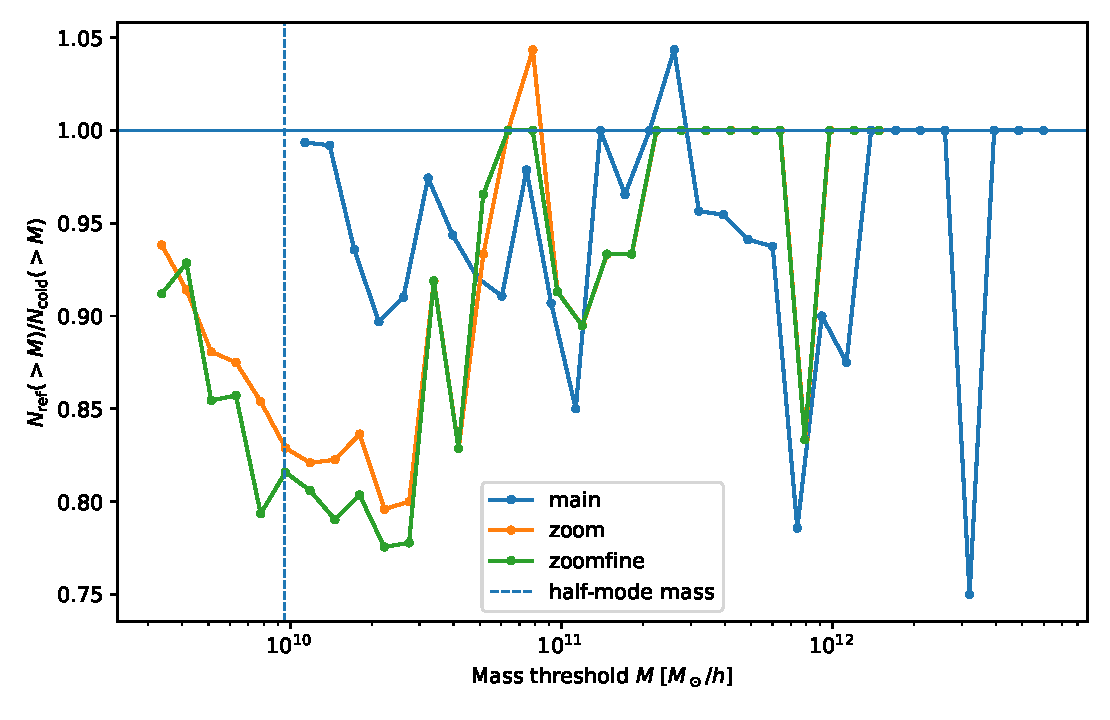
\includegraphics[width=0.86\linewidth]{figures/halo/01_cumulative_halo_abundance.pdf}
\caption{Paired cumulative halo abundance.  The vertical line is the linear half-mode mass.  Low-count high-mass points are shown for completeness but carry large finite-volume uncertainty.}
\label{fig:cumulative-halo-abundance}
\end{figure}

\section{Matched halo structure}

The zoom run yields $93$ mutual matches, of which $66$ pass the robust cut.  Their median ratios are
\begin{equation}
\boxed{
\begin{aligned}
\operatorname{med}\frac{M_{\rm ref}}{M_{\rm cold}}&=0.83371,\\
\operatorname{med}\frac{V_{\max,\rm ref}}{V_{\max,\rm cold}}&=0.94438,\\
\operatorname{med}\frac{r_{1/2,\rm ref}}{r_{1/2,\rm cold}}&=0.95535,\\
\operatorname{med}\frac{\sigma_{1\rm d,ref}}{\sigma_{1\rm d,cold}}&=0.96729.
\end{aligned}}
\label{eq:matched-halo-medians}
\end{equation}
The time-control medians are $0.82155$, $0.94496$, $0.95230$, and $0.96611$, respectively.  The median Jaccard overlap is $0.663$ in the zoom run and $0.675$ in the time control.

These results indicate that, for corresponding Lagrangian structures, refinement halos typically retain less FoF mass and a lower maximum circular-speed proxy.  The radius shift is smaller than the mass shift.  The PM force scale is too coarse for a precision concentration statement.

\begin{figure}[htbp]
\centering
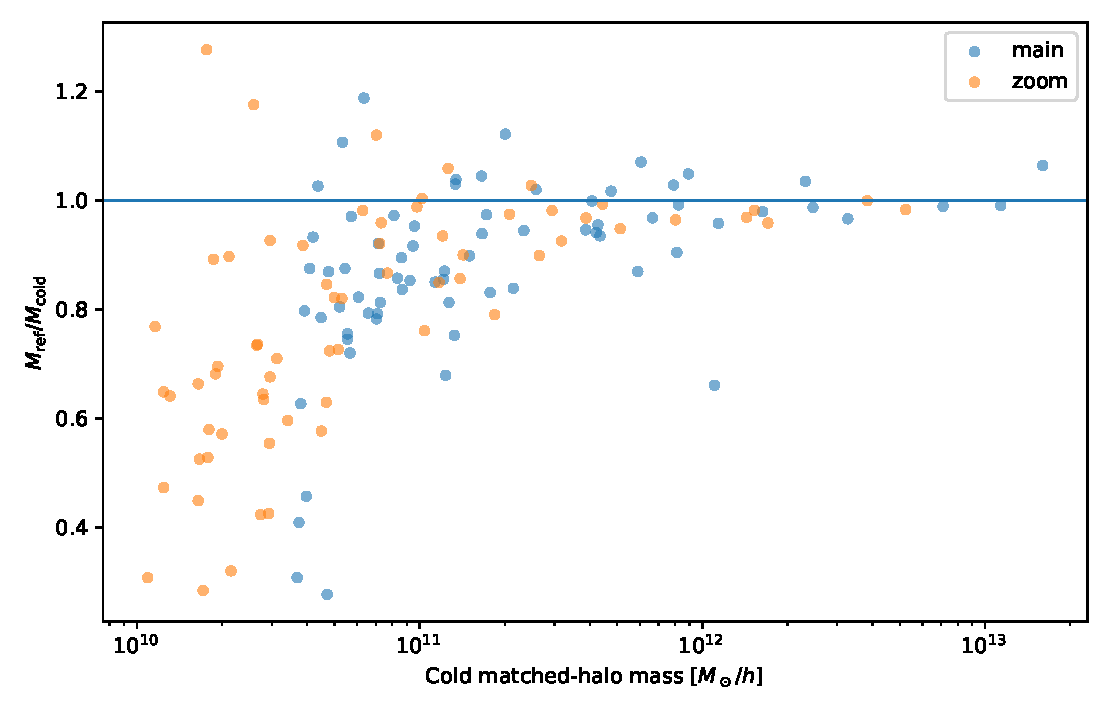
\includegraphics[width=0.84\linewidth]{figures/halo/02_matched_mass_ratios.pdf}
\caption{Particle-overlap matched halo masses.  Paired phases permit object-by-object comparison rather than comparison of two unrelated catalogues.}
\label{fig:matched-mass-ratios}
\end{figure}

\begin{figure}[htbp]
\centering
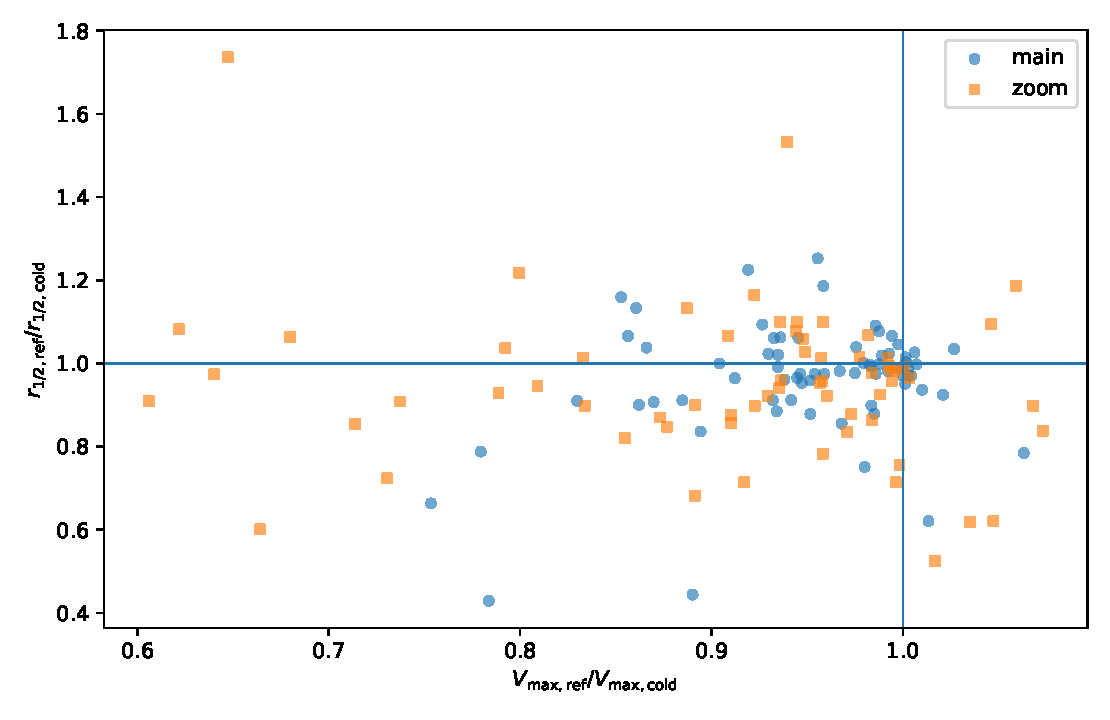
\includegraphics[width=0.78\linewidth]{figures/halo/03_matched_structure_ratios.pdf}
\caption{Matched maximum-speed and half-mass-radius proxies.  The scatter is physical, finite-resolution, and halo-finder dependent.}
\label{fig:matched-structure-ratios}
\end{figure}

\section{Assembly delay}

For the robust zoom matches, the population medians of the assembly proxy are
\begin{equation}
 \operatorname{med} f_{1/2}^{\rm cold}=0.42308,
 \qquad
 \operatorname{med} f_{1/2}^{\rm ref}=0.34836.
\label{eq:formation-population-medians}
\end{equation}
The median of the matched per-halo ratio is
\begin{equation}
\boxed{
 \operatorname{med}
 \left(
 \frac{f_{1/2}^{\rm ref}}{f_{1/2}^{\rm cold}}
 \right)
 =0.90426.}
\label{eq:formation-ratio}
\end{equation}
The $360$-step control gives $0.91483$.  Thus corresponding refinement halos have, on average, a smaller fraction of their final particles assembled into one FoF progenitor at $a=0.5$.  This is evidence for delayed assembly in the pilot, not a calibrated formation-redshift law.

\begin{figure}[htbp]
\centering
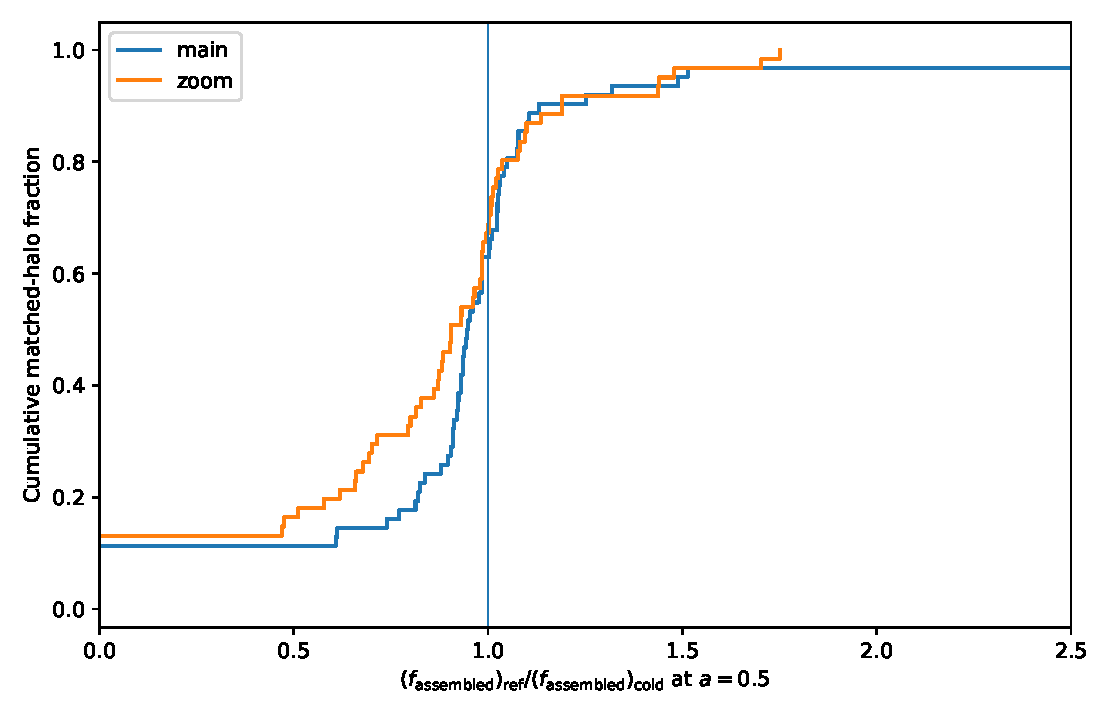
\includegraphics[width=0.80\linewidth]{figures/halo/04_formation_delay_cdf.pdf}
\caption{Cumulative distribution of the matched one-step assembly ratio.  Values below unity indicate later assembly in the refinement realization.  The horizontal range is truncated at $2.5$ so that a few small-denominator outliers do not obscure the central distribution.}
\label{fig:formation-delay}
\end{figure}

\section{Convergence and controls}

Across thresholds with at least five cold halos, the maximum difference between the $260$- and $360$-step cumulative abundance ratios is
\begin{equation}
 \epsilon_{\Delta t}=0.06042.
\label{eq:halo-time-control}
\end{equation}
At the physically central half-mode threshold the difference is only
\begin{equation}
 |0.82980-0.81507|=0.01473.
\label{eq:halo-half-mode-time-control}
\end{equation}
The maximum main-to-zoom paired-ratio discrepancy in their overlapping, count-controlled mass range is
\begin{equation}
 \epsilon_{\rm box}=0.17093.
\label{eq:halo-box-control}
\end{equation}
This includes different random phases and finite-volume effects and is not a strict spatial-convergence error.

\begin{figure}[htbp]
\centering
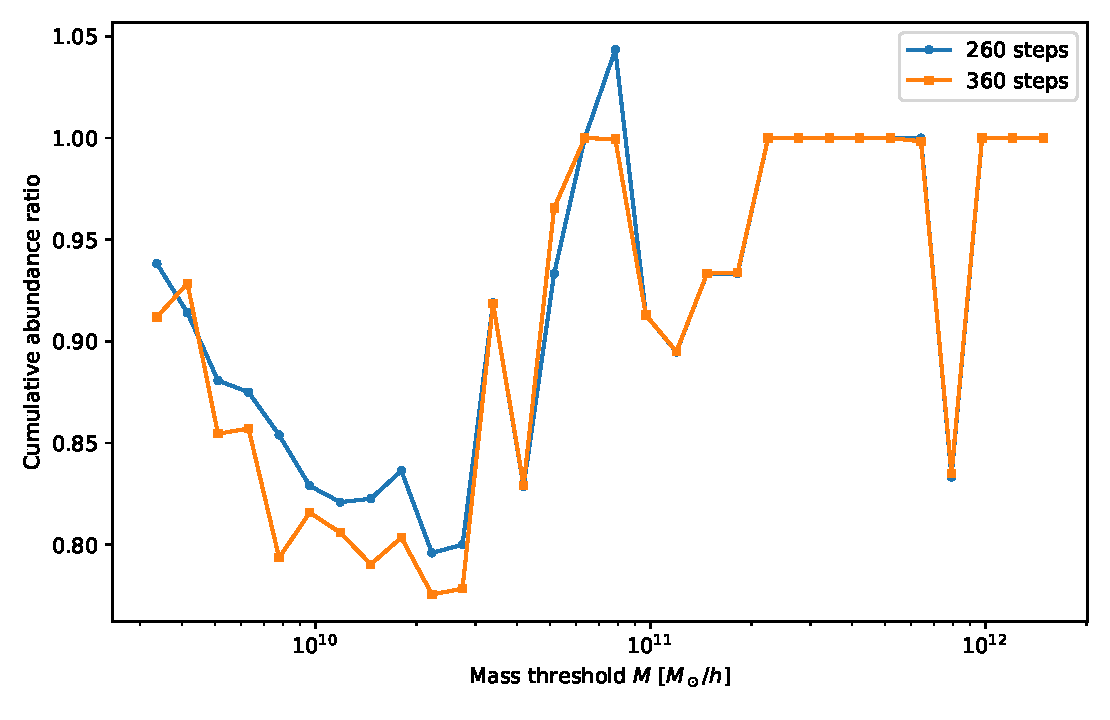
\includegraphics[width=0.82\linewidth]{figures/halo/05_time_step_control.pdf}
\caption{Time-step control in the $8\,h^{-1}\,\mathrm{Mpc}$ box.  Discrete halo counts make the curve non-smooth.}
\label{fig:halo-time-control}
\end{figure}

The deterministic audit records
\begin{equation}
\boxed{19\ \mathrm{PASS},\qquad0\ \mathrm{FAIL}.}
\label{eq:halo-audit-count}
\end{equation}
It checks nonempty catalogues, mass partition bounds, mutual matches, time and box controls, half-mode suppression, finite structural and formation ratios, label invariance, and the large-scale mass--dipole protection theorem.

\section{Physical interpretation}

The pilot sharpens the nonlinear prediction of the scale-covariant refinement dark sector:
\begin{equation}
\boxed{
\begin{aligned}
\text{large halos:}&\quad \text{approximately cold-like abundance and structure},\\
\text{near-cutoff halos:}&\quad \text{reduced abundance, mass, and }V_{\max},\\
\text{assembly:}&\quad \text{a later largest-progenitor fraction},\\
\text{two-point power:}&\quad \text{substantial nonlinear regeneration remains possible}.
\end{aligned}}
\label{eq:halo-physical-pattern}
\end{equation}
This supports the conclusion that low-mass halo counts and assembly histories retain more memory of the primordial refinement cutoff than the final nonlinear matter power alone.

\section{Claim boundary and unresolved requirements}

The calculation does not yet provide:
\begin{itemize}
\item a large-volume, high-dynamic-range halo mass function;
\item force- and particle-resolution convergence at fixed volume;
\item subhalo catalogues or converged internal density profiles;
\item baryonic hydrodynamics, cooling, star formation, or feedback;
\item a survey selection function or observational likelihood;
\item a first-principles value of the refinement mass and production scales.
\end{itemize}

A production-level nonlinear falsification test requires
\begin{equation}
\boxed{
\begin{gathered}
\text{large-volume and zoom-refined halo catalogues}\\
+\text{baryonic response envelopes}\\
+\text{frozen-parameter lensing and satellite observables}\\
\Longrightarrow
\text{first joint nonlinear falsification test}.
\end{gathered}}
\label{eq:halo-open-requirements}
\end{equation}

